\section{Polarized EMC Effect\label{sec:pemc}}
%
Since the discovery of the EMC effect~\cite{Aubert:1983xm,Bodek:1983ec} it has been clear that it embodies important new information about nuclear structure~\cite{Geesaman:1995yd}. However, this information is so well ingrained that there is as yet no consensus on what it is telling us. From one point of view it has been vigorously argued (see for example Refs.~\cite{Thomas:2016bxx,Guichon:2018uew}) that the model independent fact that there is a very strong attractive scalar mean-field in nuclei leads to changes in the internal structure of the bound nucleons, and that these changes not only explain the EMC effect but also play a vital role in the binding of atomic nuclei~\cite{Stone:2017oqt,Stone:2016qmi}. In order to distinguish between the various proposals that have been made by way of explanation for the EMC effect it is vital to find new observables which may shed light on which is correct.

One such proposal from Refs.~\cite{Cloet:2005rt,Cloet:2006bq} is to explore the spin-dependence of the EMC effect via measurement of the spin-dependent structure functions of atomic nuclei. This polarized EMC effect can be defined by:
%
\begin{align}
\Delta R_A(x) = \frac{g_{1A}(x)}{P_A^p\,g_{1p}(x) + P_A^n\,g_{1n}(x)},
\label{eq:pemc}
\end{align}
%
where $g_{1A}(x)$ is a spin-dependent nuclear structure function, $g_{1p}$, $g_{1n}$ are the free nucleon structure functions and $P_A^p$, $P_A^n$ are the effective polarization of the protons and neutrons, respectively, in a nucleus $A$. There is an approved experiment at Jefferson Lab to measure the polarized EMC effect using $^7$Li~\cite{jlabspin}, and other nuclei include $^{11}$B, $^{15}$N, and $^{27}$Al. Another promising pathway at both Jefferson Lab and an EIC would be a detailed study of the complex of polarizable nuclei: $^1$H, $^2$H, $^3$H and $^3$He.

The first calculations of the polarized EMC effect were for the hypothetical case of a polarized bound proton in nuclear matter~\cite{Cloet:2005rt}, where $g_{1A}(x) = g_{1p}^*(x)$ is the spin structure function of the bound proton which was assumed 100\% polarized ($P_A^p=1$ and $P_A^n = 0$). The effect of the medium was found to be dramatic~\cite{Cloet:2005rt} and is illustrated in the top panel of Fig.~\ref{fig:EMC_Com}, where the EMC effect was roughly twice as large for the spin-dependent case as for the unpolarized case.  For comparison, if one were to take the extreme position that all of the EMC effect arises from high momentum (highly correlated) nucleons~\cite{Weinstein:2010rt}, it seems unlikely that there would be any effect on the spin structure function.

%===============================================================================
\begin{figure}[tbp]
\centering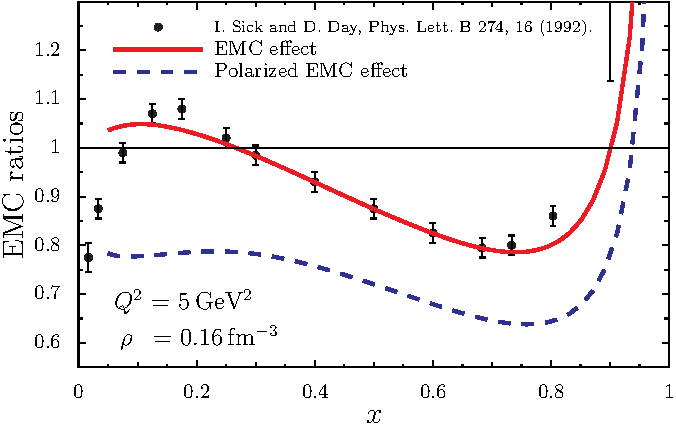
\includegraphics[width=\columnwidth]{EMCs_nuclearmatter}
\centering\includegraphics[width=\columnwidth]{EMC_Com_NLO_PDF}
\caption{{\it Top panel:} Unpolarized and polarized EMC effect results from Ref.~\cite{Cloet:2005rt}, obtained using a self-consistent NJL model calculation for nuclear matter. {\it Bottom Panel:} Analogous results from Ref.~\cite{Tronchin:2018mvu} obtained using the QMC model. In both cases the EMC data for nuclear matter is taken from Ref.~\cite{Sick:1992pw}.}
\label{fig:EMC_Com}
\end{figure}
%===============================================================================

The first calculation of the EMC effect within a self-consistent treatment of the modified structure of a bound nucleon was carried out 30 years ago using the QMC model~\cite{Thomas:1989vt}, however until very recently there had been no calculation of the polarized EMC effect within that model~\cite{Guichon:1995ue}. This is now of particular interest because it has been possible to derive an energy density functional equivalent to the QMC model, which starts with the modification of the quark structure of the nucleon in-medium, which has proven rather effective in nuclear structure studies~\cite{Guichon:2018uew,Stone:2017oqt,Stone:2016qmi}. 

Using the QMC model a calculation of the polarized EMC effect has now been completed by Tronchin {\it et al.}~\cite{Tronchin:2018mvu} and the result is reproduced in the bottom panel of Fig.~\ref{fig:EMC_Com}. We see that the prediction for the polarized EMC effect in the QMC model is about the same as that of the unpolarized effect, and a similar result was obtained in Ref.~\cite{Smith:2005ra} which used the chiral quark soliton model to perform an analogous calculation. The reason for the differences between both these calculations and the NJL result is currently not clear. However, a polarized EMC effect of the same size, or larger, than the unpolarized case would be difficult to explain using traditional nuclear structure effects or SRCs, because such an effect occurs in the valence nucleons. 

%While the consequences for the spin dependent EMC effect of a modification of nucleon structure because of the large scalar mean field in-medium are clear, the situation has been less clear for the case where SRC drive the EMC effect. 
It has been suggested in Ref.~\cite{Thomas:2018kcx} that if SRCs are indeed the sole source of the EMC effect, there should be little or no polarized EMC effect. This renders the up-coming measurement of the structure function of a polarized $^7$Li target a key test of this fundamental issue in modern nuclear physics. As explained earlier, the dominant source of high momentum nucleons in nuclei (i.e., well above the Fermi level) is tensor correlations involving a neutron-proton pair in the $^3S_1$--$^3D_1$ state. The angular momentum barrier means that the highest momentum nucleons in a correlated pair will be in $D$-wave. That is, they may meet with low relative momentum in a shell model configuration, where their relative angular momentum is $S$-wave, but through SRCs they will be scattered into a high relative momentum $D$-wave state by the tensor force. Then one can show that the effective polarization of a valence nucleon once it has scattered through a SRC into a high momentum state will be of order $-10$ to $-15$\% instead of +100\%~\cite{Thomas:2018kcx}. Thus the structure function of this weakly polarized proton cannot exhibit a strong spin dependence. 

As SRCs will depolarize the valence proton, it is clear that were the EMC-type modification of structure functions to arise {\em only} through the change of the structure function of a high momentum, far off-mass-shell nucleon in a correlated pair, there can be very little EMC effect on the nuclear spin structure functions. Once one divides the measured nuclear structure function by the effective nucleon polarization one expects little nuclear modification of the spin structure function and hence no significant spin-dependent EMC effect in this model. The polarized EMC effect is then a clear example of a major difference in the predictions of the mean-field and SRC explanations of the EMC effect.

We stress that for the polarized EMC effect results shown in Fig.~\ref{fig:EMC_Com} the proton is defined to be 100\% polarized and is embedded in nuclear matter. For a real nucleus, such as $^7$Li for which a measurement is planned at Jefferson Lab~\cite{jlabspin}, one needs to account for the reduced local density of the valence nucleons and the fact that the polarization of the bound proton is less than that of the nucleus. For the case of $^7$Li nuclear structure calculations, including varitional Monte Carlo, find $P_A^p = 0.87$ and $P_A^n = 0.04$~\cite{Pudliner:1997ck}.




